% !TEX root =  ../main_manuscript.tex 

\section{Introduction}
\label{sec:introduction}
Prostate cancer is the second most frequently diagnosed cancer in men worldwide \cite{GlobalCancerStats2012}. The increase in diagnosis of low-grade prostate cancer has been attributed to increase in life expectancy and increase in the number of screening programs \cite{potoskyPSAcancer}. An issue of prostate cancer screening programs is over‐diagnosis. To avoid further over-treatment, patients diagnosed with low-grade prostate cancer are commonly advised to join active surveillance (AS) programs. In AS, serious treatments such as surgery, chemotherapy, or radiotherapy are delayed until necessary. Instead, cancer progression is routinely examined via serum prostate-specific antigen (PSA) levels: a protein biomarker, digital rectal examination (DRE) score: a measure of the size and location of the tumor, medical imaging, and biopsies etc.

Biopsies are the most reliable prostate cancer progression examination technique used in AS. When a patient's biopsy Gleason grading becomes larger than 6, AS is stopped and patient is advised for treatment of cancer progression \cite{bokhorst2015compliance}. Since biopsies are invasive they are conducted intermittently, until cancer progression is detected. Consequently, progression is always detected with a delay, equal to the difference between the time of the last biopsy and the unobserved true time of progression. Biopsies are also painful, and prone to medical complications \cite{ehdaie2014impact}. Hence, the decision of conducting a biopsy requires a fine compromise between the burden incurred due to biopsies and the delay in detection of progression. However, currently there is no consensus on the best time interval for subsequent repeat biopsies \cite{loeb2014heterogeneity}. Many AS programs focus on minimizing only the delay, by scheduling biopsies annually \cite{welty2015extended}. Annual biopsies may work well for patients who progress fast, but for slowly progressing patients many unnecessary burdensome biopsies are scheduled. To improve the share of burden between fast and slow progressing patients, the world's largest AS program Prostate Cancer Research International Active Surveillance (PRIAS) \cite{bul2013active}, schedules annual biopsy only if at a follow-up visit a patient has a PSA doubling time between 0 and 10 years. PSA doubling time is measured as the inverse of the slope of the regression line through the base two logarithm of the observed PSA values. For everyone else, PRIAS schedules biopsies at following fixed follow-up times: year 1, 4, 7, and 10, and every 5 years thereafter. Despite this effort, in PRIAS over a period of 10 years a patient may get scheduled for 4 to 10 biopsies. Consequently, patients may not always comply with the schedule \cite{bokhorst2015compliance}. This can lead to the original problem of delayed detection of prostate cancer progression, and reduce the effectiveness of AS.
\begin{figure}[!htb]
\captionsetup{justification=justified}
\centerline{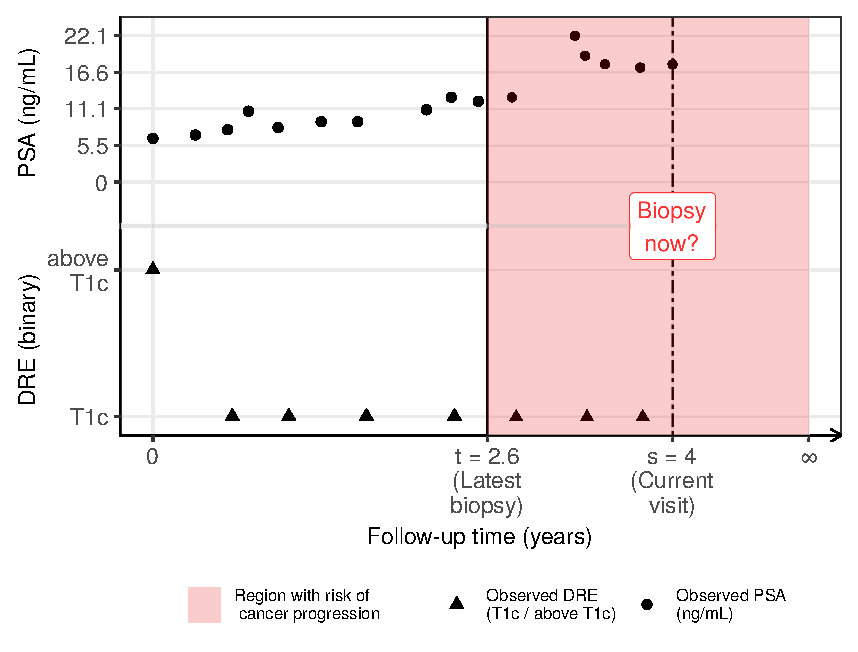
\includegraphics[width=\columnwidth]{images/obsDataPlot_2340.eps}}
\caption{Illustration of the problem of making a decision for conducting biopsy at a follow-up visit ($s=3.96$ years). No cancer progression is detected at the latest biopsy ($t=2.55$ years). The goal is to detect cancer progression as soon as possible after it happens, by conducting a biopsy. The shaded region shows the time period in which the patient is at the risk of cancer progression. We utilize the entire history of PSA and DRE measurements along with the time of latest biopsy up to a follow-up visit to make the decision of biopsy at that visit.}
\label{fig:obsDataPlot_2340}
\end{figure}

This article is motivated by the need to better balance the number of biopsies and the delay in detection of prostate cancer progression, than in practice currently. We intend to achieve this by personalizing the decision of conducting biopsies at follow-up visits (see Figure \ref{fig:obsDataPlot_2340} for illustration). Personalized decision making has received much interest in the literature, especially for various cancers. For example, Markov decision process (MDP) models have been used to create personalized screening schedules for breast cancer \cite{ayer2012or}, cervical cancer \cite{akhavan2017markov}, and colorectal cancer \cite{erenay2014optimizing}. In the specific case of prostate cancer, Zhang et al. \cite{zhang2012optimization} have used partially observable MDP models to personalize the decision of (not) deferring a biopsy to the next check‐up time during the screening process. This decision is based on the baseline characteristics as well as a discretized PSA level of the patient at the current screening-visit time.

In comparison to the work referenced above, we do not base the decision of biopsy only on the current PSA value, but instead we utilize the entire history of PSA values, DRE scores, and results of the latest biopsy. To this end, we employ joint models for time-to-event and longitudinal data \cite{tsiatis2004joint,rizopoulos2012joint}. Since joint models use random effects \cite{laird1982random} to model the between-patient heterogeneity, they are inherently patient-specific. Using joint models we first obtain a full specification of the joint distribution of the time of cancer progression, and PSA and DRE measurements. We then use it separately for each patient at each follow-up visit to define a visit and patient-specific posterior predictive distribution of the time of cancer progression, given the observed PSA and DRE measurements, and time of the latest biopsy up to that visit. We calculate the patient's risk of cancer progression at the follow-up visit using this distribution. If the risk is higher than a certain threshold our method schedules a biopsy at the same follow-up visit. Since there is no clear consensus on such risk thresholds we not only use fixed thresholds suggested by urologists, but also present a methodology to automate the choice of thresholds. 

To develop our methodology we rely on the PRIAS dataset. However, biopsies are already conducted for PRIAS patients according to the PRIAS schedule. In addition, the cancer progression times of patients are observed with interval and right censoring. Given these reasons, and the ethical issues with testing new methods of biopsies on real patients, it is not possible to evaluate our methodology on real patients. Instead, to reliably evaluate our methodology we conduct an extensive simulation study. In the simulation study we compare the personalized approach with the annual and PRIAS schedules. For a realistic comparison, we utilize an exact replica of the population of the PRIAS patients, generated using the model fitted to the PRIAS dataset. 

The rest of the article is structured as follows: The details of the joint modeling framework and biopsy decision making methodology are presented in detail in the \hyperref[sec:methods]{Methods} section. The details of the simulation study and the corresponding results are presented in \hyperref[sec:methods]{Methods} and \hyperref[sec:results]{Results} sections, respectively.